\documentclass[a4paper, 12pt]{report}

%%%%%%%%%%%%
% Packages %
%%%%%%%%%%%%

\usepackage[english]{babel}
\usepackage[noheader]{packages/sleek}
\usepackage{packages/sleek-title}
\usepackage{packages/sleek-theorems}
\usepackage{packages/sleek-listings}
\usepackage{amsmath}
%%%%%%%%%%%%%%
% Title-page %
%%%%%%%%%%%%%%

\logo{./resources/image/UJM_logo.png}
\institute{Jean Monnet University}
\faculty{Computational Colour and Spectral Imaging (COSI)}
%\department{Department of Anything but Psychology}
\title{Computer Vision}
\subtitle{Camera Calibration - Lab 2}
\author{\textit\\Gemal Hamid \textsc{Hisuin}}
%\supervisor{Linus \textsc{Torvalds}}
%\context{Well, I was bored...}
\date{\today}

%%%%%%%%%%%%%%%%
% Bibliography %
%%%%%%%%%%%%%%%%

\addbibresource{./resources/bib/references.bib}

%%%%%%%%%%
% Others %
%%%%%%%%%%

\lstdefinestyle{latex}{
    language=TeX,
    style=default,
    %%%%%
    commentstyle=\ForestGreen,
    keywordstyle=\TrueBlue,
    stringstyle=\VeronicaPurple,
    emphstyle=\TrueBlue,
    %%%%%
    emph={LaTeX, usepackage, textit, textbf, textsc}
}

\FrameTBStyle{latex}

\def\tbs{\textbackslash}

%%%%%%%%%%%%
% Document %
%%%%%%%%%%%%

\begin{document}
    \maketitle

\textcolor{red}{ \textbf{Description:} \newline
The objective of this exercise session is to learn and perform camera calibration using MATLAB and CalTech
calibration toolboxes.
As a part of this lab session you will do the following task sequentially:
• Learn the basic usage of a famous camera calibration toolboxes.
• Calibrate single camera using the toolbox.
• Calibrate a stereo system the toolbox.
}
\newline
\section{Introduction}

 Camera Calibration is an estimation of the intrinsic and extrinsic parameters of a camera needed to identify an accurate relationship between a real-world 3D point and their respective 2D projection. Radial distortion and tangential distortion are two main distortions caused by pinhole cameras. Straight lines appear curved because of radial distortion. Similarly, the tangential distortion occurs because the imaging lens is not perfectly aligned with the image plane. Single camera Calibration and/or stereo camera calibration is necessary when: we develop a computer stereo vision, and when it is necessary to correctly measure the planar objects with an accurate estimate of the camera parameters. The images captured are affected with radial and/or tangential distortion, and the camera calibration techniques are used to remove them. \newline \newline
 A selection window that looks like figure 1.1 appears by running the main matlab calibration function "calib gui.
 \newline 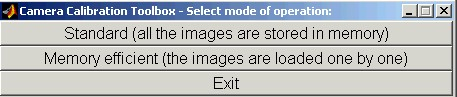
\includegraphics[width=1.0\textwidth]{resources/image/1.jpg} \newline 
 Figure 1.1: Selection window \newline \newline 
 Figure 1.1 will help us select between the toolbox's two modes of operation: standard and memory efficient. If the images are big, a memory-efficient version of the toolbox is preferred. However, in this session, I would use standard mode so all of the images used for calibration will be loaded into memory once and never read from disk again, which will have an advantage of minimizing the total amount of disk accesses and better speed during the image processing. \newline
 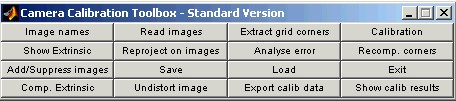
\includegraphics[width=1.0\textwidth]{resources/image/2.jpg} \newline
 Figure 1.2: Standard mode \newline
  \section{First Calibration Example}
To calibrate a single camera, we need at least two images to get the parameters. If we already have a single camera calibrated, we can use one pair of checkerboard image to get R and T, but it is not very precise. Since we need enough images to cover the field of view and to have a good 3D orientation distribution, it’s usually advisable if one single camera is calibrated using 10 to 20 image pairs. In this course-based lab work, I have used a CalTech camera calibration MATLAB tool with 20/25 images for single camera calibration.
   \subsection{Procedure of Calibration}
The key objective in this example is to calibrate one camera with different CalTech features that mainly serve to load calibration images, extracting corners, displaying results, adding and suppressing images, and exporting calibration data in various formats. 

 \newline \newline
\textbf{1:} Using the ‘Image names’ function on the tool, I loaded 20 images with a .tif file extension and then stored the images.\newline 
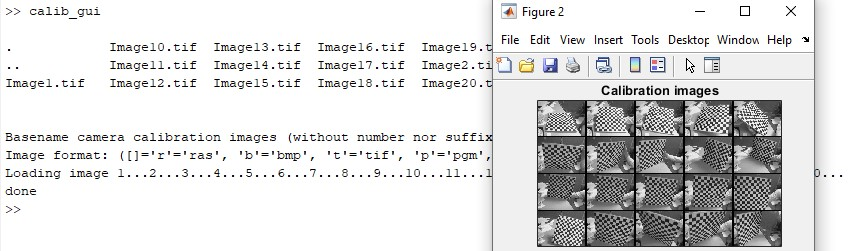
\includegraphics[width=1.0\textwidth]{resources/image/4.jpg} \newline
Figure 1.3: Calibration images \newline \newline 
\textbf{2:} : I extracted the grid corners for 15 images from the checkboard image using the feature ‘Extract grid corners'. \newline
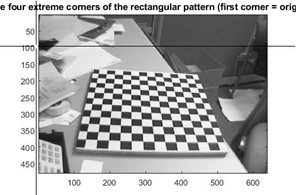
\includegraphics[width=0.8\textwidth]{resources/image/5.jpg} \newline
Figure 1.4: First calibration image \newline
By clicking at four different corners in the image we detect the boundary of the calibration grid. The first clicked point is then chosen, and it is aligned with the starting point of the reference frame connected to the grid. This first-click rule is particularly important when we have to calibrate several cameras. \newline
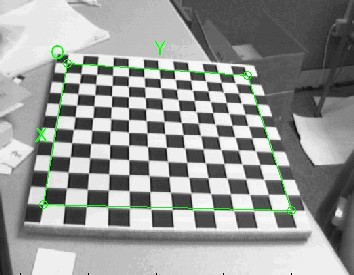
\includegraphics[width=0.9\textwidth]{resources/image/6.jpg} \newline
Figure 1.5: Boundary of calibration grid \newline \newline 
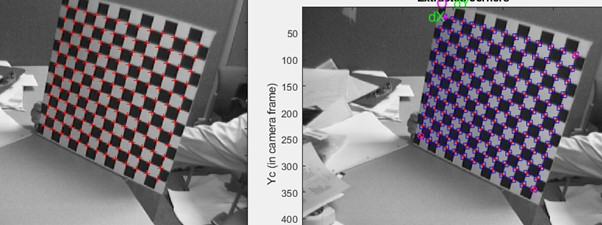
\includegraphics[width=0.9\textwidth]{resources/image/8.jpg} \newline \newline 
Figure 1.6: Predicted grid corner (Accurate) \newline \newline 
The results for most of the images indicate that the predicted corners are close to the actual image corners, which shows that there is no distortion, and that the prediction is accurate. However, for two images, image 15 and image 18 the predicted corner was not close to the true image corners due to the presence of an image distortion, and the predicted corner for those two images is later refined with radial distortion coefficient values to obtain accurate corners.\newline 
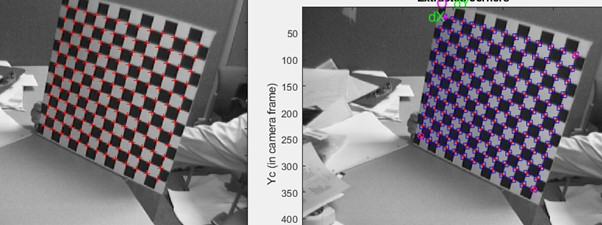
\includegraphics[width=0.9\textwidth]{resources/image/8.jpg} \newline 
Figure 1.7: Inaccurate image corner prediction (left). Accurate corner prediction after applying distortion coeffiecient (right).\newline \newline 
For all 20 images, I followed the same method of extraction. But I didn't use the predictive distortion function on (16-20) images. In fact, I only found image 18 with a prediction inaccuracy. \newline \newline \newline 
\textbf{Step 3:} [main calibration phase]: The calibration procedure is divided into two steps: initialization and non-linear optimization. The user manually selects four extreme corners of the grid during the initialization process. The initialization step determines a closed form solution with no lens included for calibration parameters. The non-linear optimization step minimizes the total reprojection factor for all calibration parameters (9 degree of freedom (DOF) for intrinsic parameters and 120 degree of freedom (DOF) for extrinsic parameters). The optimized projection matrix minimizes the sum of all grid corner reprojection errors.
\newline
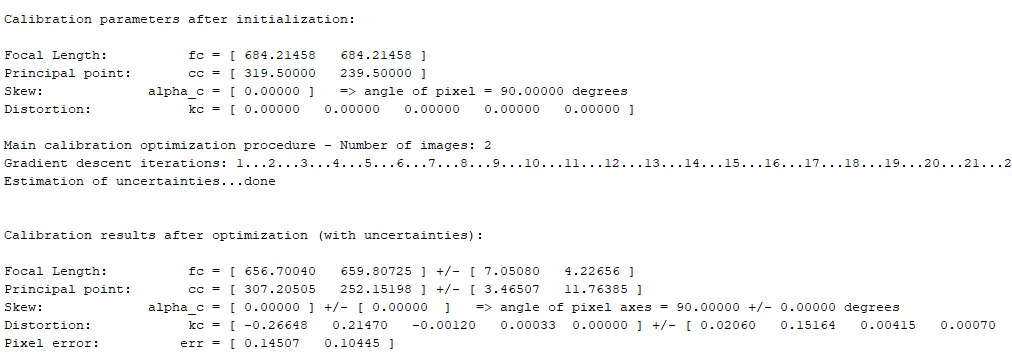
\includegraphics[width=1.2\textwidth]{resources/image/21.jpg} \newline
The corresponding calibration matrix K is given by: \newline
 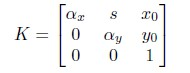
\includegraphics[width=0.3\textwidth]{resources/image/22.jpg} \newline
Where alpha\_x alpha\_y are the focal length,  alpha\_x=656.70040   alpha\_y=659.80725 \newline
s is the skew factor, s=0.0000 \newline 
and x0 and y0 are the principal points. x0=307.20505, x0=252.1598
\newline 
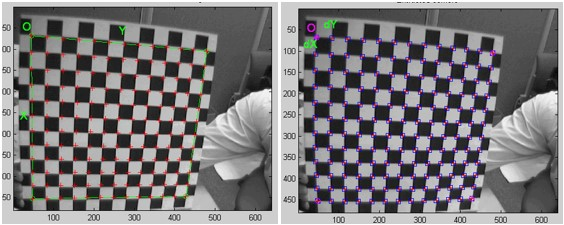
\includegraphics[width=1.0\textwidth]{resources/image/9.jpg} \newline 
Figure 1.8: Detected corner (red crosses) and the reprojected grid corners (circles) \newline \newline 

\textbf{4:} As some images have not been extracted very well from the grid corners, the reprojection error is too high to allow an assessment of the model's complexity. \newline 
To display grids on the original image reprojections and to determine these projections on the basis of the current intrinsic and extrinsic parameters. I have measured the reprojection error corresponding to the image distance between a projected and a measured point and quantify how close a 3D point estimate recreates the true projection of the point.
\newline
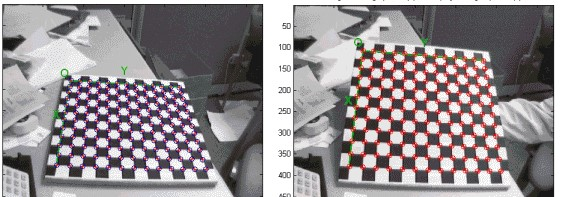
\includegraphics[width=1\textwidth]{resources/image/10.jpg} \newline
Figure 1.9: Reprojection error and Extrinsic parameters \newline \newline
Since I did not do an effective analysis of extracting corners from the highly distorted images, we can see from the error plot that there is a major reprojection error through the figures. However, by adjusting the size of the corner finder window, I will now be able to fix the corners on all images using the function "Recomp. Corners" tool. After optimization, the calibration data including the intrinsic and extrinsic parameters are saved. \newline 
Then, after reprojecting the grids into original images with the "Reproject on images" function, I found that the error in the current projection is much smaller than before. \newline 
By using the ‘Calibration' function, we can run another calibration optimization. During the calibration the standard deviation of the reprojection error (in pixel) is calculated in both the x and y directions, and the uncertainties in the calibration parameters are measured with numerical values approximately three times the standard deviations. \newpage
Window size 5 \newline 
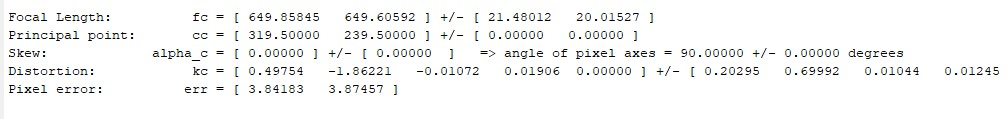
\includegraphics[width=1.0\textwidth]{resources/image/im8n.jpg} \newline
Calibration parameters reveal a significant decrease in pixel error after reextracting corners with corner finder window size set to 1.\newline 
 Pixel error has been redistributed uniformly between x and y. \newline 
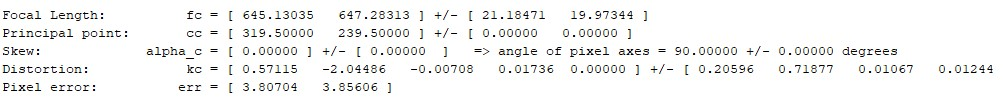
\includegraphics[width=1.2\textwidth]{resources/image/im8_f1.jpg} \newline

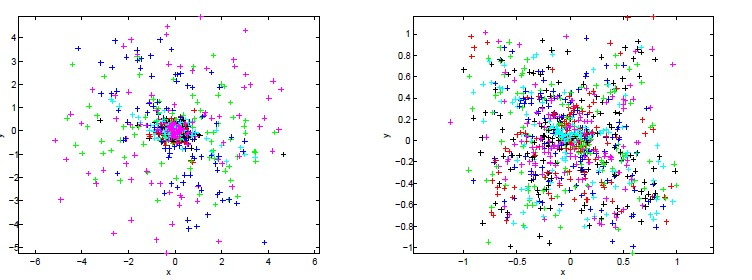
\includegraphics[width=1.0\textwidth]{resources/image/24.jpg} \newline
Figure 2.1: Reprojection error before and after refining the plot  \newline

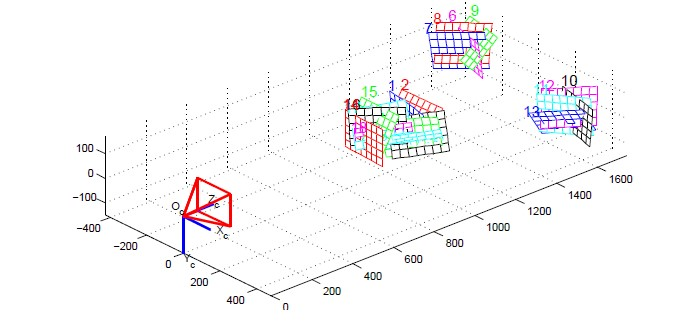
\includegraphics[width=1.1\textwidth]{resources/image/26.jpg} \newline
Figure 2.: Position of grids \newline \newline 
The new reprojection error reveals that the error is significantly less than before. \newline \newline 
Also with distortion coefficient we can also minimize the error.
 \newline 
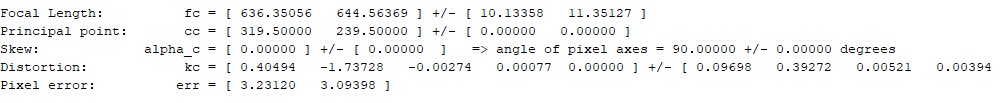
\includegraphics[width=1.2\textwidth]{resources/image/im6n.jpg}
\newline

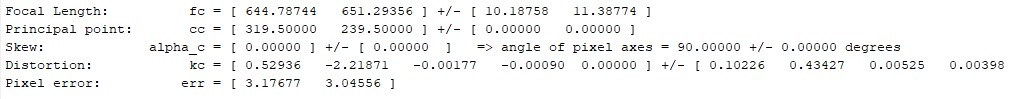
\includegraphics[width=1.2\textwidth]{resources/image/im6_k.5.jpg} \newline
Figure 2.: Minimized calibration error using Kc=0.5 \newline \newline 
The error inspection tool is very useful in cases where the corners have been badly extracted on one or several images. In such a case, the user can recompute the corners of the specific images using a different window size (larger or smaller). \newline 
For the second and third calls of ‘Recomp. Corners’, using wintx=winty=8 for image 18 and wintx=winty=7 for images 5, 7, 8, and 19 in automatic mode. The result implies that the reprojection error is somewhat smaller than the previous one. Furthermore, the uncertainties in the calibration parameters are reduced. \newline 
Window size 5x5 \newline 
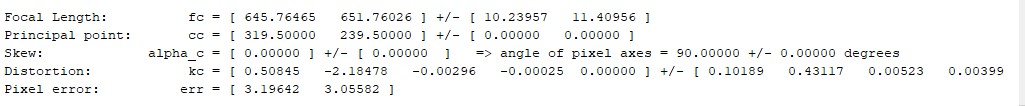
\includegraphics[width=1.2\textwidth]{resources/image/im81n.jpg}
\newline
window size 8x8 \newline
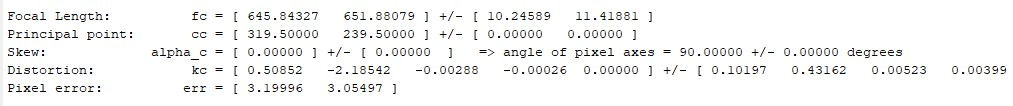
\includegraphics[width=1.2\textwidth]{resources/image/im8_w8.jpg} \newline
\textbf{5:} By saving five more images to the current directory. I re-calibrate the camera using the full set of 25 images without re-calibrating everything from scratch. \newline 

The corners of the five new images were extracted, with the default window sizes wintx=winty=5. \newline 
With three ‘Recomp. corners’ and using different window size, the four last image corners were recomputed. For images 22 and 24 wintx=winty=9 and wintx=winty=8 is used for image 23 and wintx=winty=6 for image 25. After that, new calibration results with the intrinsic and extrinsic parameters are estimated.
We perform the calibration between the angle x and y pixel axes by using the skew factor alpha\_c. To achieve this, we set the variable est\_alpha to one. \newline
I have found that the skew coefficient is very close to zero after optimization. This results in an angle of almost 90 degree between the x and y pixel axes.   Moreover, I notice that there is great ambiguity with the radial distortion coefficient of the sixth order. In such cases, the calculation should be disabled. \newline 
Since the effect of distortions on the pixel image is important to visualize, by using the script ‘visualize\_distortions’ at MATLAB prompt we can make the decision on a suitable distortion model to visualize the full radial and tangential distortion of each pixel of the image. I noticed that points in the image corners were displaced by 25 pixels and, in the entire distortion model, it was also possible to remove the tangential distortion quite well.
\newline 
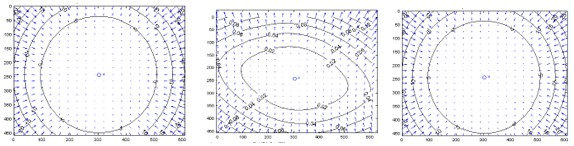
\includegraphics[width=0.9\textwidth]{resources/image/15.jpg} \newline
Figure 2.4: Complete, Tangential Component and Radial Component Distortion Models \newline \newline 
By setting the est\_aspect\_ratio, center\_optim, est\_dist and est\_alpha  all to 0, we can run a calibration that rejects the aspect ratio fc(2)/fc(1), the principal point cc, the distortion coefficients kc, and the skew coefficient alpha c from the optimization measurement. Also, the best approximation for its position would be at the center of the image if the principal point cc is not estimated. To ensure that the principal point cc is still at the center of the image after optimisation, a new optimisation can be done by clicking on the ‘Calibration’. \newline 

\section{Fifth Calibration Camera}
\subsection{Stereo Calibraiton}

In this section, I've seen how stereo system calibration (intrinsically and extrinsically) works with CamTool support, and how to use stereo calibration, stereo image rectification and 3D stereo triangulation.\newline
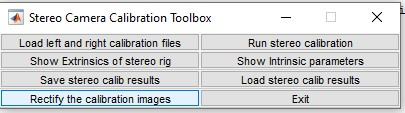
\includegraphics[width=0.9\textwidth]{resources/image/17.jpg} \newline
Figure 3.1: Stereo camera calibration tool \newline \newline 
In this case, 14 sets of the corresponding left and right images have been used. The package contains two separate calibration results files, Calib\_Results\_left.mat and Calib\_Results\_right.mat, created using the standard methodology (the first example) after calibration of two different cameras. \newline 
The outcome of the "load left and right calibration files" shows the stereo calibration parameters of the intrinsic camera[focal length, principal point, skew and distortion] of left and right cameras, and estimates for the extrinsic parameters OM and T that characterize the relative position of the right camera with respect to the left camera. \newline 
After global stereo optimization is called using the “Run stereo calibration” tool, the reprojection errors on both camera are reduced at all positions of the grid. I have observed that along with all complexities, all intrinsic and extrinsic parameters were recomputed. Furthermore, since global stereo optimization takes place through a few unknown parameters, the intrinsic parameters (especially those of focal values) for both cameras are less uncertain following stereo calibration and this reveals that the structure's global rigidity moves from left to right. \newline \newline
Results after loading individual calibration files: \newline  \newline 
Left camera: \newline 
Focal length: [595.75748. 595.91958]
Principal point: [327.84526 244.88635]
Skew: 0
Distortion: [-0.18032 2.7854 0.00391 -0.00912 0]
\newline 
Right Camera: \newline 
Focal length: [794.42301 796.52413]
Principal point: [260.12035 247.99523]
Skew:0
Distortion: [-0.08465 0.27451 0.00059 -0.00607 0]
\newline 
Rotation vector: [-0.06327 0.84210 0.02963] \newline 
Translation vector: [-761.02416 70.92541 1041.021542]
\newline \newline 
Results after stereo optimization \newline 
Left camera \newline 
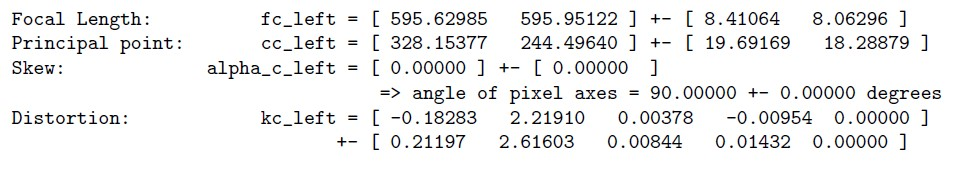
\includegraphics[width=0.9\textwidth]{resources/image/44.jpg} 
\newline 
Right camera \newline 
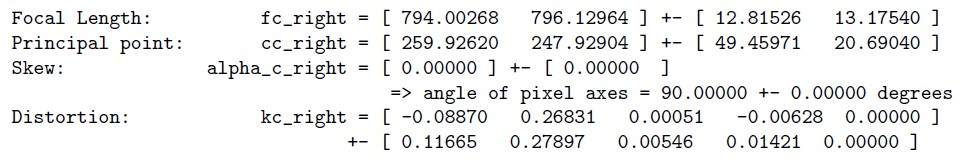
\includegraphics[width=1.0\textwidth]{resources/image/45.jpg} \newline 
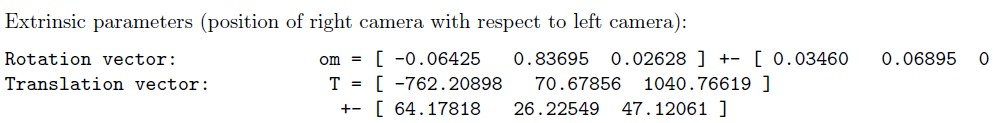
\includegraphics[width=1.0\textwidth]{resources/image/35.jpg} 
\newline 
\textit{Note: I have tested the calibration in two different phases with two different image datasets. The above calibration result of stereo calibration is from the images other than the ones given on the documentation's official website.)} \newline 
The om rotation vector is a co-directional vector with the axis of rotation, and whose magnitude is identical to the angle of rotation. The rotation matrix is obtained using Rodrigues formula. \newline 
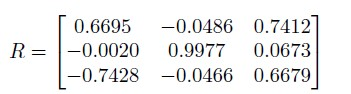
\includegraphics[width=0.4\textwidth]{resources/image/30.jpg} \newline 
Using "Show Extrinsics of the stero rig" function the spatial structure of the two cameras and the calibration planes are shown in a 3D format. \newline
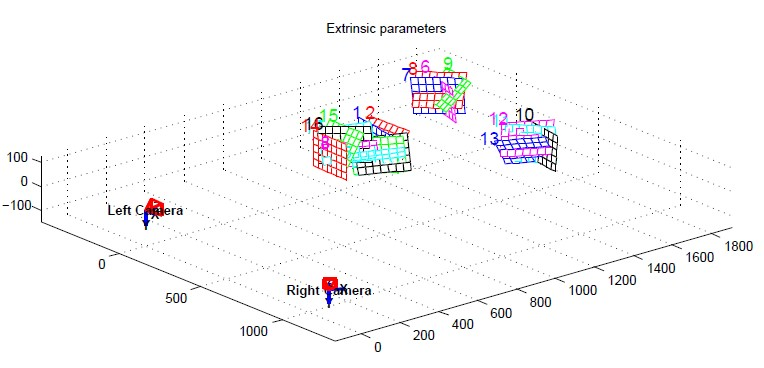
\includegraphics[width=0.9\textwidth]{resources/image/str.jpg} \newline 
Figure 3.2: Stereo rig spatial configuration \newline 
\subsection{Stereo Rectification}
Image rectification makes use of epipolar information, which reduces the correspondence problem to a 1D search. The idea is that any couple of images can be transformed in parallel camera geometry such that the corresponding point features in 3D are placed in both images along the same horizontal axis. \newline 
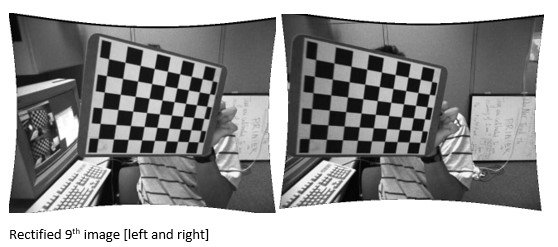
\includegraphics[width=0.71\textwidth]{resources/image/60.jpg}  \newline
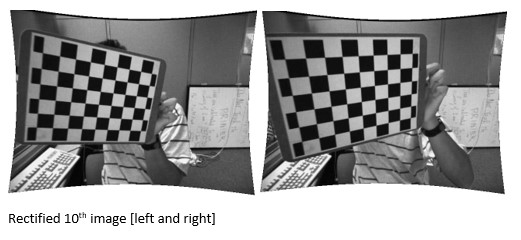
\includegraphics[width=0.71\textwidth]{resources/image/61.jpg} \newline 
Figure 3.7: Stereo Rectification \newline \newline 
\textit{NB: My MATLAB crashes when I draw the line (I have no idea why is that :))). However, on the final rectified image, there should be an epipolar line between the left and right images.}\newpage

\subsection{Stereo Triangulation}
The MATLAB function 'stereo\_triangulation.m' is useful to calculate the 3D position of a series of points given their left and right image projections. As the relative position and orientation of the two cameras is identified, we can establish the 3D position of point P from the perspective projection of P on the camera image plane. After the left camera is chosen as a 3D reference system, the right camera has been translated and rotated with respect to left camera. Besides, the optimal path of stereo triangulation happens where the optical axis of the two cameras is parallel and the translation of the right camera is around the X axis. \newline 
Let's assume with projection matrix P=[I | 0]. Point in space is mapped to: \newline 
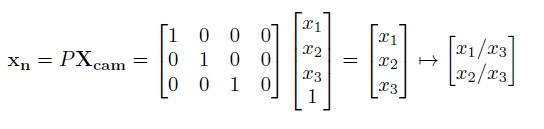
\includegraphics[width=0.5\textwidth]{resources/image/36.jpg} \newline 
xn is a normalized image point that corresponds to a ray in 3D space on which Xcam is located. 
We may use the normalized coordinates for each camera to construct the ray that starts at the camera center and ends at point X. The intersection of these two rays will be at X. Thus, using the normalized coordinates of the representations in a stereo rig, we were able to determine the 3D coordinates of a point in space.
\newline 
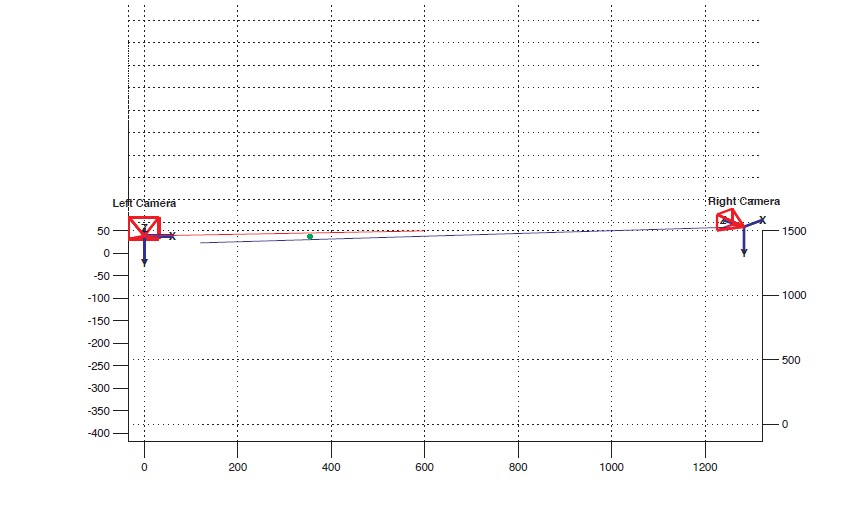
\includegraphics[width=1.0\textwidth]{resources/image/37.jpg} \newline 
Figure 3.8: left and right camera rays [do not intersect]
\newline \newline
A point can be located in 3D world coorganizations by doing a stereo triangulation on the images of a point from a pair of calibrated stereo images.\newline
(Note): The same set of points must be chosen in the left and right images during the corner extraction process. This implies that using the same grid of points and the same origin point is helpful in ensuring an identical pattern reference frame. \newline 



\section{References}
[1] \url{http://www.vision.caltech.edu/bouguetj/calib_doc/htmls/example.html} \newline
[2] \url{http://www.vision.caltech.edu/bouguetj/calib_doc/htmls/example5.html}\newline
[3] \url{http://www.vision.caltech.edu/bouguetj/calib_doc/htmls/parameters.html}

\end{document}
